% CV in LaTeX
\documentclass[12pt,oneside]{article} % article with 12pt font

%% PACKAGES %%

\usepackage[english]{babel} % multilingual support
\usepackage[utf8]{inputenc} % encoding
\usepackage{blindtext} % to insert blind text
\usepackage{tgpagella} % Set the default font
\usepackage{graphicx} % Set the default font
%\usepackage{showframe}% http://ctan.org/pkg/showframe
%\usepackage{eso-pic}% http://ctan.org/pkg/eso-pic
\usepackage[all]{background}
\usepackage{tikz}

% set the page layout
\usepackage{geometry}
\geometry{
	a4paper,
	left=15mm,
	right=15mm,
	bottom=0mm,
	top=10mm}

% empty the headers, footers, pagenumbers…
\pagestyle{empty}

% Custom sectioning with secsty
\usepackage{sectsty}

\sectionfont{
	\large % make sections smaller
	\fontfamily{qag}\selectfont % change font family
	\sectionrule{0pt}{0pt}{-5pt}{1pt} % insert a thin rule
}

%% MACROS %%

% size of the boxes used to align text
\newlength{\spacebox}
\settowidth{\spacebox}{123456789}

% vertical space separator between entries
\newcommand{\sepspace}{\vspace*{1em}}

% name
\newcommand{\name}[1]{
\Huge % font size
\fontfamily{phv}\selectfont % font family
% print name centered and bold
\begin{center} \textbf{#1} \end{center}\par
% back to normal size and font
\normalsize\normalfont}

% motto
\newcommand{\motto}[1]{
	\large % font size
	\fontfamily{phv}\selectfont % font family
% print motto centered and slanted
	\begin{center} \textsl{#1}\end{center}\par
% back to normal size and font
	\normalsize \normalfont}
	
	% personal information
\newcommand{\info}[2]{
% set specific indentation for personal information
	\noindent\hangindent=2em\hangafter=0
% create a box to align two pieces of text
	\parbox{\spacebox}{%
	\textsl{#1}} % slanted entry name
	#2 \par} % entry value
	
	% skill
\newcommand{\skill}[2]{
% set specific indentation for personal information
\noindent\hangindent=2em\hangafter=0
% create a box to align two pieces of text
\parbox{3\spacebox}{% three times larger box
\textsc{#1}} % small caps entry name
#2 \par} % entry value

% language level
\newcommand{\lan}[2]{
	% set specific indentation for personal information
	\noindent\hangindent=2em\hangafter=0
	% create a box to align two pieces of text
	\parbox{2\spacebox}{%
		\textbf{#1}} % bold font entry name
	 #2 \par}    % entry value

% education entry
\newcommand{\education}[4]{

% name of the studies
\noindent  \textbf{#1}
% at the right the duration
	\hfill 
	\framebox{% duration inside a frame box
	\parbox{6em}{%
	\centering\textbf{#2}}} \par

 % new paragraph with the school in italics
	\noindent \textit{#3} \par
	% description with no hanging and in smaller text
	\vspace*{0.5em}
	\noindent\hangindent=2em\hangafter=0 \small #4
%back to normal size
\normalsize \par}

% work experience

\newcommand{\work}[4]{
% name of the work
  \noindent  \textbf{#1}
% at the right the duration
  \hfill 
\framebox{% duration inside a frame box
  \parbox{6em}{%
  \centering\textbf{#2}}} \par
% new paragraph with the school in italics
  \noindent \textit{#3} \par
% description with no hanging and in smaller text
  \vspace*{0.5em}
  \noindent\hangindent=2em\hangafter=0 \small #4
%back to normal size
\normalsize \par}

\newcommand{\MyGraphicLogo}{% For imported graphic logo
\begin{tikzpicture}[remember picture,overlay,yshift=-3cm, xshift=-3.5cm]
  \node at (0,0) {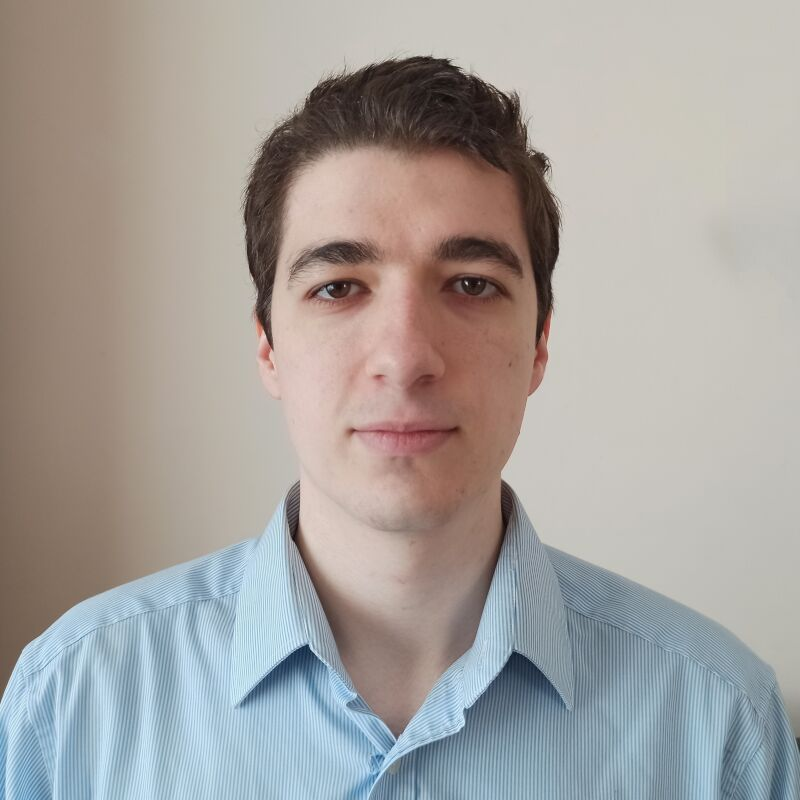
\includegraphics[width=4cm]{komolybab_kicsi.jpg}};
 \end{tikzpicture}
}

\SetBgContents{\MyGraphicLogo}% Select included image

\SetBgPosition{current page.north east}% Select location
\SetBgOpacity{1.0}% Select opacity
\SetBgAngle{0.0}% Select roation of logo
\SetBgScale{1.0}% Select scale factor of logo

\begin{document}
% name and motto
\name{Gábor Szilágyi}
%\vspace*{-10pt}
%\motto{Work is my motivation}

% personal information
%\sepspace
\info{Email}{\texttt{gbr.szilagyi@gmail.com}}
\info{Phone}{+36 30 756 8542}
\info{Address}{1032 Budapest, Kiscelli utca 16, 7/40}
\info{Birth}{1999.05.18.}

% education
\section*{Education}

\education{Master's Degree in Electrical Engineering (in progress)}{2022--2024}{Budapest University of Technology and Economics}{Department of Broadband Infocommunications and Electromagnetic Theory\\FPGA Based Systems (auxiliary specialization) \vspace{2ex}}

\education{Bachelor's Degree in Electrical Engineering}{2018--2022}{Budapest University of Technology and Economics}{Department of Broadband Infocommunications and Electromagnetic Theory}

% work experience
\section*{Work Experience}

\work{Hardware Intern}{2021--2022}{Silicon Laboratories Hungary kft.}{
\begin{itemize} \setlength\itemsep{0.5ex}
	\item Radiated/conducted RF measurements at the on-site antenna chamber
	\item Soldering tasks (mostly fine-tuning of matching/filter networks)
	\item PCB design in Altium, Schematic/BOM management
	\item Python programming for measurement automation
	\item Printed antenna design and simulation in AWR Microwave Office and CST
\end{itemize}}

% technical skills
\section*{Technical skills}

\skill{Programming languages}{\textsc{C}, \textsc{C++}, \textsc{MATLAB}, \LaTeX, \textsc{Python}, \textsc{Rust}}
\skill{Other}{\textsl{Git, Vim, Linux, Amateur Radio lincense, Neural Networks}}

% languages
\section*{Languages}
\lan{Hungarian}{native}
\lan{English}{C1}

% Social competencies
\section*{Social competencies}
\begin{itemize} \setlength\itemsep{0.5ex}
	\item I consider myself very empathic
	\item Experience as the team leader of the HA5KFU amateur radio club in the Simonyi Károly Szakkollégium
	\item I can work efficiently both in teams and alone
\end{itemize}
\end{document}